\documentclass{article}

\usepackage[letterpaper]{geometry}
\usepackage{tgpagella}
\usepackage{amsmath}
\usepackage{amssymb}
\usepackage{amsthm}
\usepackage{tikz}
\usepackage{minted}
\usepackage{physics}
\usepackage{siunitx}
\usepackage{revsymb}

\sisetup{detect-all}
\newtheorem{plm}{Problem}
\renewcommand*{\proofname}{Solution}

\title{4721 HW 6}
\author{Duncan Wilkie}
\date{6 April 2023}

\begin{document}

\maketitle

\begin{plm}
  Common forms assumed for the momentum distributions of valence quarks in the proton are:
  \[
    F_{u} = xu(x) = a(1 - x)^{3}, \; F_{d}(x) = xd(x) = b(1 - x)^{3}.
  \]
  If the valence quarks account for half of the proton's momentum---i.e.
  \[
    \int_{0}^{1}xu(x)dx + \int_{0}^{1}xd(x)dx = \frac{1}{2},
  \]
  find the values of $a$ and $b$.
  Hint: the $u$ quarks carry approximately twice as much momentum as the $d$ quarks in the proton.
\end{plm}

\begin{proof}
  Some calculus:
  \[
    \int_{0}^{1}(1 - x)^{3}dx = \int_{1}^{0}u^{3} \cdot -du = \frac{u^{4}}{4}\eval_{u=0}^{u=1} = \frac{(1 - x)^{4}}{4}\eval_{x=1}^{x=0}
    = \frac{1}{4}
  \]
  Accordingly,
  \[
    \int_{0}^{1}xu(x)dx + \int_{0}^{1}xd(x)dx = \frac{1}{2}
    \Leftrightarrow a\int_{0}^{1}(1 - x)^{3}dx + b\int_{0}^{1}(1 - x)^{3}dx = \frac{1}{2}
    \Leftrightarrow \frac{a}{4} + \frac{b}{4} = \frac{1}{2}
    \Leftrightarrow a + b = 2.
  \]
  There are two valence up quarks, and one valence down quark, so one would expect the total momentum in the up quarks to be double
  that of the down quark---accordingly,
  \[
    2b + b = 2 \Leftrightarrow b = \frac{2}{3} \Rightarrow a = \frac{4}{3}.
  \]
\end{proof}

\begin{plm}
  What is the color wavefunction for mesons, in analogy to that for baryons of
  \[
    y_{baryon} = y_{space}y_{spin}(rgb + gbr + brg - rbg - bgr - grb)?
  \]
  Explain your answer.
\end{plm}

\begin{proof}
  This baryon color wavefunction comes from noticing that baryons are made up of three quarks, all of different color charge
  (so as to produce a color-neutral baryon), and then requiring the resulting wavefunction to be antisymmetric under particle interchange,
  so as to produce a fermionic composite particle.
  By contrast, mesons are bosonic, and so the color wavefunction must stay the same under particle interchange:
  \[
    y_{meson} = y_{space}y_{spin}\qty(r\bar{r} + g\bar{g} + b\bar{b}).
  \]
\end{proof}

\begin{plm}
  The diagram below shows the internal gluon interactions in a proton.
  Complete the diagram by labelling the color of the quarks and gluons.
\end{plm}

\begin{proof}
  The governing principle is that the net color of the proton is always white.
  \begin{center}
    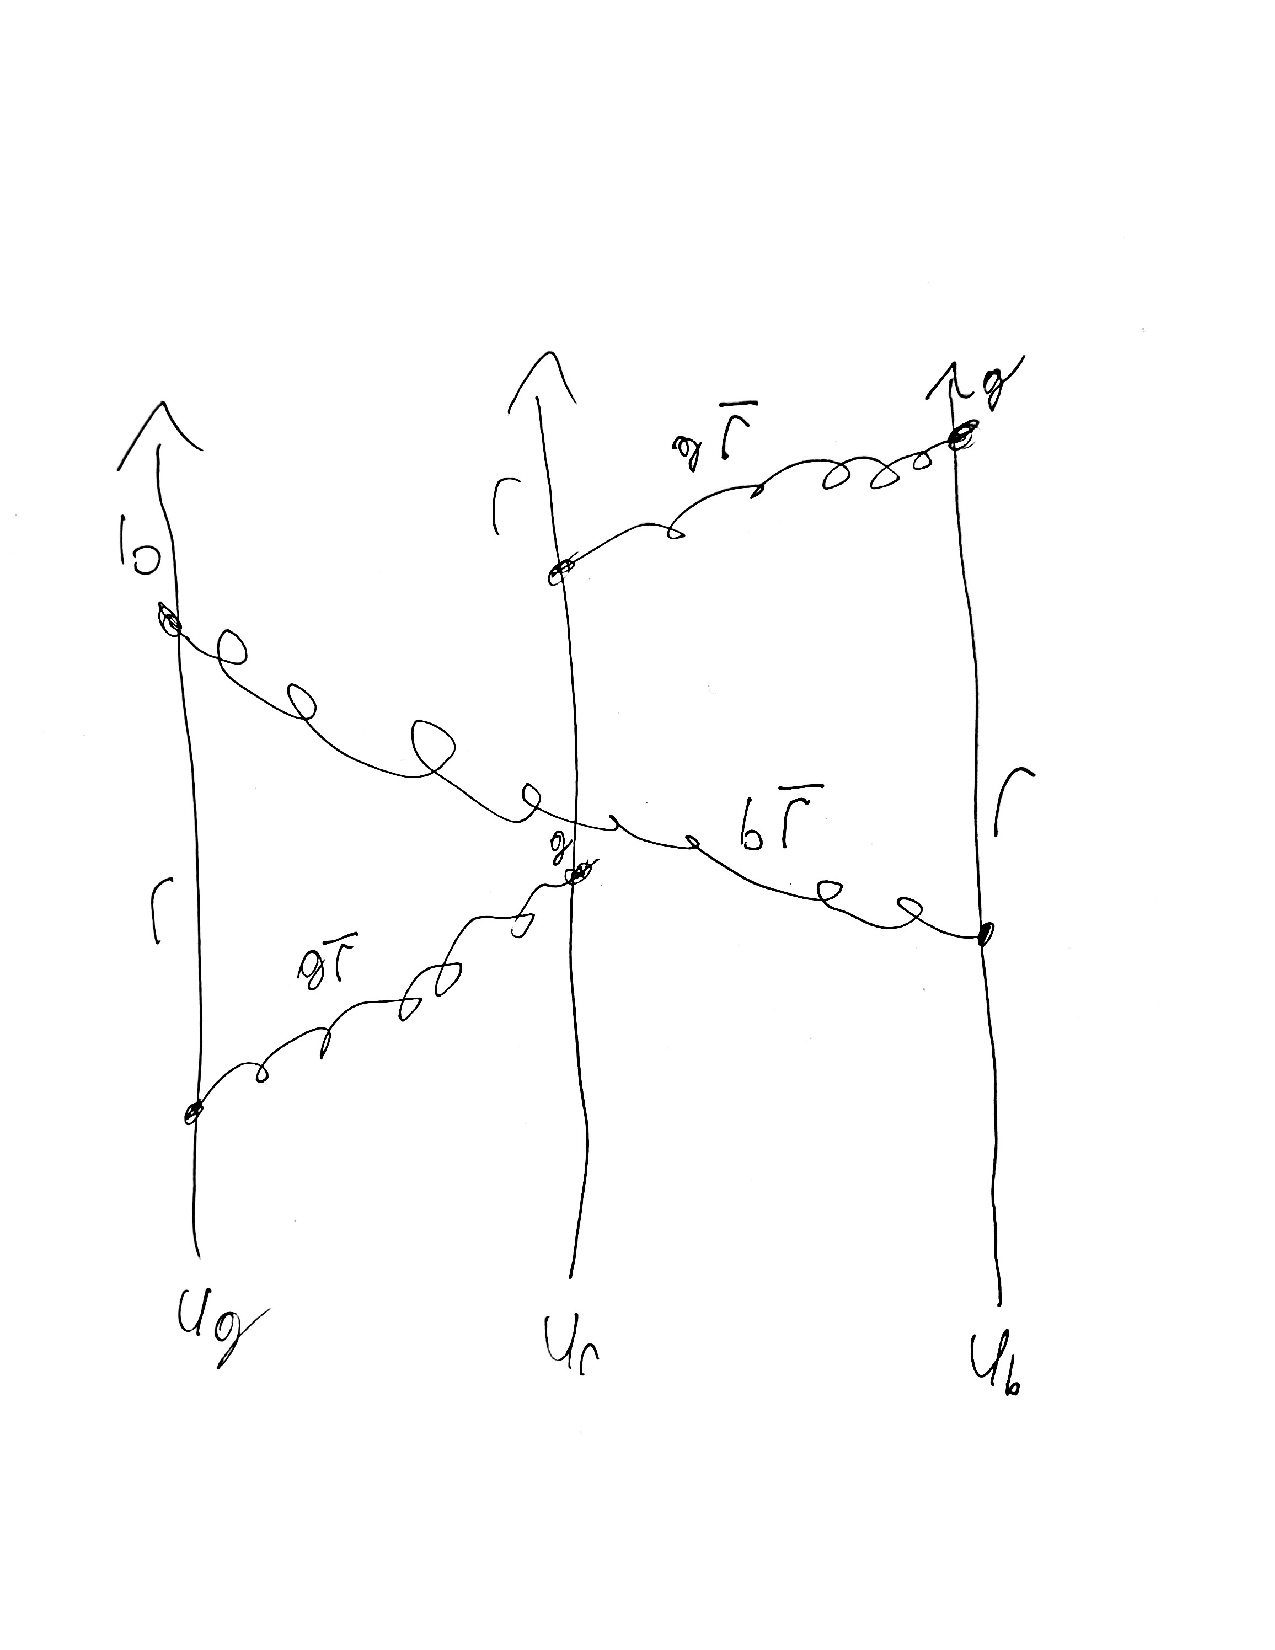
\includegraphics[scale=0.3]{gluon_exchange.pdf}
  \end{center}
  Note that I accidentally copied down the quark types incorrectly; the rightmost trajectory should be a down quark, of course.
\end{proof}

\begin{plm}
  Which of the following processes are allowed?
  If not allowed, state why.
  If allowed, say whether the process is strong, weak, or electromagnetic.
  \begin{enumerate}
  \item $\nu_{e} + p \to e^{-} + \pi^{+} + p$
  \item $e^{+} + e^{-} \to \mu^{+} + \mu^{-}$
  \item $\Sigma^{-} \to n + \pi^{-}$
  \item $\bar{\nu}_{e} + p \to e^{-} + n$
  \item $e^{-} + p \to \nu_{e} + \pi^{0}$
  \end{enumerate}
\end{plm}

\begin{proof} \;
  \begin{enumerate}
  \item Allowed; weak.
  \item Allowed; electromagnetic.
  \item Allowed; strong.
  \item Disallowed; charge changes.
  \item Disallowed; baryon number changes.
  \end{enumerate}
\end{proof}

\begin{plm}[Double Points]
  The differential cross section for $e^{+} + e^{-} \to \mu^{+} + \mu^{-}$ is given by
  \[
    \dv{\sigma}{\Omega} = \frac{\alpha^{2}}{4s}(\hbar c)^{2}(1 + \cos^{2}\theta)
  \]
  in a collider experiment where $s = 4E_{e}$ and $E_{e}$ is the electron/positron energy.
  \begin{enumerate}
  \item Integrate over the solid angle to obtain an expression for the total cross section.
  \item If you use an electron beam energy of \SI{4}{GeV}, what rate of production of $\mu^{+}\mu^{-}$ would you expect at a luminosity of
    \SI{e33}{Hz/cm^{2}}?
  \item Calculate the ratio of the hadronic production cross section to that for $\mu^{+}\mu^{-}$ at $E_{e} = \SI{500}{GeV}$.
    If you use an electron beam energy of \SI{500}{GeV}, what must the luminosity be to measure the hadronic cross section within 24 hours
    with 10\% statistical uncertainty?
  \end{enumerate}
\end{plm}

\begin{proof} \;
  \begin{enumerate}
  \item We have a total cross-section
    \[
      \int \dv{\sigma}{\Omega} d\Omega = \int_{0}^{2\pi}\int_{0}^{\pi}\frac{\alpha^{2}}{4s}(\hbar c)^{2}\qty(1 + \cos^{2}\theta)\sin\theta
      d\theta d\phi
      = \frac{2\pi(\alpha\hbar c)^{2}}{4s}\int_{0}^{\pi}\sin\theta + \sin\theta\cos^{2}\theta d\theta
    \]
    \[
      = \frac{\pi(\alpha\hbar c)^{2}}{2s}\qty(2 - \int_{1}^{-1}u^{2}du)
      = \frac{\pi(\alpha\hbar c)^{2}}{2s}\qty(2 + \frac{u^{3}}{3}\eval_{-1}^{1})
      = \frac{\pi(\alpha\hbar c)^{2}}{2s}\qty(2 + \frac{2}{3})
      = \frac{4\pi(\alpha\hbar c)^{2}}{3s}
    \]
  \item If the electron beam energy is \SI{4}{GeV}, $s = 4 \cdot E_{e} = \SI{16}{GeV}$, and at the given luminosity,
    the expected production rate is
    \[
      L \cdot \sigma = \SI{e33}{Hz/cm^{2}} \cdot \frac{4\pi\qty(\frac{1}{137} \cdot \SI{3.16e-24}{J \cdot cm})^{2}}
      {3 \cdot \SI{16}{GeV} \cdot \SI{1.6e-19}{J/GeV}}
      = \SI{8.71e-10}{Hz}
    \]
  \item The cross-section ratio is, if the Standard Model's accounting of quarks is correct, should be $\frac{11}{3}$---a
    \SI{500}{GeV} beam is well beyond the $Z$ production threshold, so all quark types will be produced (including the top quark).
    Accordingly, the expected hadronic cross section would be
    \[
      \sigma_{h} = R\sigma_{\mu\mu} = \frac{15}{3} \cdot \frac{4\pi \qty(\frac{1}{137} \cdot \SI{3.16e-24}{J \cdot cm})^{2}}
      {3 \cdot \SI{500}{GeV} \cdot \SI{1.6e-19}{J/GeV}}
      = \SI{1.39e-43}{cm^{2}}
    \]
    As this is a count data experiment, the observed hadron production rate is the parameter of the Poisson distribution
    associated with the Poisson process of the number of hadrons produced.
    The sampling distribution from a Poisson distribution has standard deviation $\sqrt{\frac{\lambda}{n}}$,
    for a sample of $n$ counts.
    This estimates the uncertainty in a post-hoc parameter estimation of $r_{h}$, given our prediction above.
    The uncertainty in the entailing estimate of $\sigma_{h}$ is, by error propagation on the formula $\sigma_{h} = \frac{r_{h}}{L}$,
    \[
      \frac{1}{L}\sqrt{\frac{r_{h}}{n_{h}}}
    \]
    However, $n_{h}$ and $r_{h}$ we can estimate in advance as $n_{h} = \sigma_{h}Lt$ and $r_{h} = \sigma_{h}L$;
    we therefore have an estimated uncertainty
    \[
      \frac{1}{L}\sqrt{\frac{\sigma_{h}L}{\sigma_{h}Lt}} = \frac{1}{L\sqrt{t}}.
    \]
    A 10\% margin around the expected value of $\sigma_{h}$ would be $\pm \SI{1.39e-44}{cm^{2}}$, so equating this to the above,
    \[
      \SI{1.39e-44}{cm^{2}} = \frac{1}{L\sqrt{t}} \Leftrightarrow L = \frac{1}{\SI{1.39e-44}{cm^{2}} \cdot \sqrt{\SI{24}{hr}}}
      = \SI{2.54e41}{Hz/cm^{2}}
    \]
  \end{enumerate}
\end{proof}

\begin{plm}[Double Points]
  In an $e^{+}e^{-}$ collider experiment, a resonance $R$ is observed at $E_{cm} = \SI{10}{GeV}$ in both the $\mu^{+}\mu^{-}$
  and hadronic final states.
  The integrated cross sections are
  \[
    \int \sigma_{\mu \mu}(E)dE = \SI{10}{nb \cdot GeV}
  \]
  and
  \[
    \int \sigma_{h}(E)dE = \SI{300}{nb \cdot GeV}.
  \]
  Use a Breit-Wigner form for the resonance production to deduce the partial widths $\Gamma_{\mu\mu}$ and $\Gamma_{h}$ in \si{MeV}
  for the decays $R \to \mu^{+}\mu^{-}$ and $R \to \text{hadrons}$.
  Assume the integral
  \[
    \int_{resonance}\frac{dE}{(E - Mc^{2}) + \Gamma^{2}/4}dE \approx \frac{2\pi}{\Gamma}.
  \]
\end{plm}

\begin{proof}
  The Breit-Wigner resonance formula for a particular decay channel gives
  \[
    \sigma_{f} = \frac{3\pi\lambdabar^{2}}{4} \cdot \frac{\Gamma_{i}\Gamma_{f}}{(E - E_{r})^{2} + \Gamma_{T}^{2}/4}
  \]
  Accordingly, the integrated cross-section is expected to be
  \[
    \int\sigma_{f} dE = \frac{3\pi\lambdabar^{2}}{4} \cdot \frac{2 \pi \Gamma_{i}\Gamma_{f}}{\Gamma_{T}}
    = \frac{3\pi^{2}\lambdabar^{2}}{2} \cdot \frac{\Gamma_{i}\Gamma_{f}}{\Gamma_{T}}
    = \frac{3\lambda^{2}}{8} \cdot \frac{\Gamma_{i}\Gamma_{f}}{\Gamma_{T}}
  \]
  For the two decays in question, presuming they are the only relevant channels,
  \[
    \frac{3\lambda^{2}}{8} \cdot \frac{\Gamma_{e^{+}e^{-}}\Gamma_{\mu\mu}}{\Gamma_{T}} = \SI{10}{nb \cdot GeV}
  \]
  \[
    \frac{3\lambda^{2}}{8} \cdot \frac{\Gamma_{e^{+}e^{-}}\Gamma_{h}}{\Gamma_{T}} = \SI{300}{nb \cdot GeV}
  \]
  \[
    \Gamma_{T} = \Gamma_{\mu\mu} + \Gamma_{h}
  \]
  We can compute, in the relativistic approximation,
  \[
    \lambda = \frac{h}{p} = \frac{h}{E/c} = \frac{\SI{4.13e-15}{eV \cdot s}}{\SI{10}{GeV} / \SI{3e8}{m/s}}
    = \SI{1.239e-16}{m}
    \Rightarrow \frac{3\lambda^{2}}{8} = \SI{5.76e-33}{m^{2}} = \SI{57.6}{\micro\barn}
  \]
  Three equations, four unknowns; simplifying and substituting,
  \[
    \frac{\Gamma_{e^{+}e^{-}}\Gamma_{\mu\mu}}{\Gamma_{\mu\mu} + \Gamma_{h}} = \SI{17.4}{MeV}
  \]
  \[
    \frac{\Gamma_{e^{+}e^{-}}\Gamma_{h}}{\Gamma_{\mu\mu} + \Gamma_{h}} = \SI{5.21}{MeV}.
  \]
  Taking the ratio,
  \[
    \frac{\Gamma_{\mu\mu}}{\Gamma_{h}} = \frac{\SI{17.4}{MeV}}{\SI{5.21}{MeV}} = 3.34
    \Leftrightarrow \Gamma_{\mu\mu} = 3.34\Gamma_{h}.
  \]
  Substituting,
  \[
    \Gamma_{e^{+}e^{-}} = (1 + 3.34)\SI{5.21}{MeV} = \SI{22.61}{MeV}.
  \]
  Try as I might, I cannot reduce further; all I get is different forms of the linewidth ratio expressed above
  (which is just the expected $10/3$).
\end{proof}

\begin{plm}
  Find the threshold kinetic energy for each of the following reactions, assuming the first particle to be incident on the second particle
  at rest:
  \begin{enumerate}
  \item $K^{-} + p \to \Xi^{-} + K^{+}$
  \item $\bar{p} + p \to \Upsilon$
  \item $\pi^{-} + p \to \omega + n$
  \end{enumerate}
\end{plm}

\begin{proof}
  For all these calculations, we transform into the center-of-mass frame and apply the conservation of energy equation;
  in each case, the velocity of the initial particles is the same, and the velocity of the produced particles is zero in this frame.
  Then, we perform velocity addition on the particle that's supposed to move in the lab frame to obtain its velocity;
  the lab-frame beam kinetic energy is then immediate.
  Masses are read from the Particle Data Group tables.
  \begin{enumerate}
  \item We have
    \[
      \gamma m_{K^{-}}c^{2} + \gamma m_{p}c^{2} = m_{\Xi^{-}}c^{2} + m_{K^{+}}c^{2}
      \Leftrightarrow \gamma = \frac{m_{\Xi} + m_{K}}{m_{K} + m_{p}}
      \Leftrightarrow \frac{v}{c} = \sqrt{1 - \qty(\frac{m_{K} + m_{p}}{m_{\Xi} + m_{K}})^{2}}
    \]
    \[
      = \sqrt{1 - \qty(\frac{\SI{494}{MeV/c^{2}} + \SI{938}{MeV/c^{2}}}{\SI{1321}{MeV/c^{2}} + \SI{494}{MeV/c^{2}}})^{2}}
      = 0.61
    \]
    Using velocity addition, one gets an incoming $K^{-}$ velocity of
    \[
      v = \frac{2v_{cm}}{1 + v_{cm}^{2}/c^{2}} = \frac{2 \cdot 0.61c}{1 + (0.61c)^{2}/c^{2}} = 0.896c
    \]
    corresponding to an energy of
    \[
      E = \gamma m_{K^{-}}c^{2} = \frac{\SI{494}{MeV/c^{2}} \cdot c^{2}}{\sqrt{1 - (0.896c)^{2}/c^{2}}}
      = \SI{2.5}{GeV},
    \]
    or a kinetic energy of
    \[
      K = E - m_{K^{-}}c^{2} = \SI{2.5}{GeV} - \SI{494}{MeV} = \SI{2}{GeV}
    \]
  \item We have
    \[
      \gamma m_{\bar{p}}c^{2} + \gamma m_{p}c^{2} = m_{\Upsilon}c^{2}
      \Leftrightarrow \gamma = \frac{m_{\Upsilon}}{m_{\bar{p}} + m_{p}}
      \Leftrightarrow \frac{v}{c} = \sqrt{1 - \qty(\frac{m_{\bar{p}} + m_{p}}{m_{\Upsilon}})^{2}}
    \]
    \[
      = \sqrt{1 - \qty(\frac{\SI{938}{MeV/c^{2}} + \SI{938}{MeV/c^{2}}}{\SI{9.46}{GeV/c^{2}}})^{2}}
      = 0.98
    \]
    Using velocity addition, one gets an incoming $K^{-}$ velocity of
    \[
      v = \frac{2v_{cm}}{1 + v_{cm}^{2}/c^{2}} = \frac{2 \cdot 0.98c}{1 + (0.98c)^{2}/c^{2}} = 0.9994c
    \]
    corresponding to an energy of
    \[
      E = \gamma m_{\bar{p}}c^{2} = \frac{\SI{494}{MeV/c^{2}} \cdot c^{2}}{\sqrt{1 - (0.99994c)^{2}/c^{2}}}
      = \SI{4}{TeV},
    \]
    with respect to which the proton mass is a rounding error, so the kinetic energy will be the same.
  \item We have
    \[
      \gamma m_{\pi^{-}}c^{2} + \gamma m_{p}c^{2} = m_{\omega}c^{2} + m_{n}c^{2}
      \Leftrightarrow \gamma = \frac{m_{\omega} + m_{n}}{m_{\pi^{-}} + m_{p}}
      \Leftrightarrow \frac{v}{c} = \sqrt{1 - \qty(\frac{m_{\pi^{-}} + m_{p}}{m_{\omega} + m_{n}})^{2}}
    \]
    \[
      = \sqrt{1 - \qty(\frac{\SI{140}{MeV/c^{2}} + \SI{938}{MeV/c^{2}}}{\SI{783}{MeV/c^{2}} + \SI{940}{MeV/c^{2}}})^{2}}
      = 0.76
    \]
    Using velocity addition, one gets an incoming $K^{-}$ velocity of
    \[
      v = \frac{2v_{cm}}{1 + v_{cm}^{2}/c^{2}} = \frac{2 \cdot 0.76c}{1 + (0.76c)^{2}/c^{2}} = 0.96c
    \]
    corresponding to an energy of
    \[
      E = \gamma m_{\pi^{-}}c^{2} = \frac{\SI{140}{MeV/c^{2}} \cdot c^{2}}{\sqrt{1 - (0.96c)^{2}/c^{2}}}
      = \SI{1.85}{GeV},
    \]
    or a kinetic energy of
    \[
      K = E - m_{\pi^{-}}c^{2} = \SI{1.85}{GeV} - \SI{140}{MeV} = \SI{1.71}{MeV}.
    \]
  \end{enumerate}
\end{proof}

\end{document}
